\documentclass[ecta,nameyear,draft]{econsocart}
\usepackage{amsmath,amsfonts,amssymb,amsthm,booktabs,array,longtable}
\usepackage{graphicx}
\usepackage[T1]{fontenc}
\usepackage{mathpazo,microtype,needspace,xurl}
\usepackage{xr-hyper}
\RequirePackage[colorlinks,citecolor=blue,linkcolor=blue,urlcolor=blue]{hyperref}
\startlocaldefs
\newtheorem{theorem}{Theorem}
\newtheorem{proposition}[theorem]{Proposition}
\newtheorem{lemma}[theorem]{Lemma}
\newtheorem{corollary}[theorem]{Corollary}
\newcommand{\E}{\mathbb E}
\newcommand{\R}{\mathbb R}
\endlocaldefs
\setlength{\emergencystretch}{3em}
\makeatletter\def\copyright@text{Prepared for referee review}\makeatother

\setcounter{secnumdepth}{2}

% Stable current-document identity for clean typesetting reproduction.
\ifdefined\pdfinfoomitdate\pdfinfoomitdate=1\fi
\ifdefined\pdfsuppressptexinfo\pdfsuppressptexinfo=15\fi
\ifdefined\pdftrailerid\pdftrailerid{}\fi

\externaldocument[][nocite]{build/supp}[supp.pdf]
\externaldocument[][nocite]{build/appendix}[appendix.pdf]
\begin{document}
\begin{frontmatter}
\title{Neural Bellman Operators}
\runtitle{Neural Bellman Operators}
\begin{aug}
\author[id=au1,addressref={add1}]{\fnms{Qian}~\snm{QI}\ead[label=e92ECTA]{qiqian@pku.edu.cn}}
\address[id=add1]{Peking University}
\end{aug}
\begin{abstract}
Neural Bellman Operators construct and learn continuations for feasible decisions
under a specified recursive economic objective. We connect their own-future
policy account to action-dependent error, continuous-risk information and
complete computational cost. For a convex Lipschitz continuation under uniform
innovations, locating the adverse tails before integration gives matching
deterministic point-information bounds of order $KR(1-\alpha)N^{-2}$, with
risk-level-uniform constants. An outward original-model tail defect and global
action supports yield a certificate for the implemented complete policy.
A bounded prelude and packed evaluation make this information account
operational before an unchanged complete fallback. Original Bellman foundations,
constrained gradients, signed policy comparisons and recursive-utility boundary
conditions receive full proofs. Separate frozen comparisons retain all neural,
hinge, polynomial, spline, semi-analytic and grid controls, original-policy
reference enclosures and actual failed or adverse evidence. Packing improves 10 of 16 contemporaneous median service-time cells against
the geometric control, while every service returns the same original policy.
The quadratic representation remains a complete-cost and economic winner
in the reported catalogue. These results separate original economic gains
from implementation savings and identify action-aligned learning and
matched-cost adoption as the next substantive NBO questions.
\end{abstract}
\begin{keyword}
\kwd{Dynamic programming}\kwd{Neural approximation}\kwd{Recursive risk}
\kwd{Policy qualification}\kwd{Computational economics}
\end{keyword}
\end{frontmatter}
\section{Introduction}\label{sec:intro119}
Dynamic investment under risk requires a continuation value, a feasible action,
and a decision about how much information to acquire before acting. A small
continuation fitting error need not imply a small decision loss. It can move a
nearly binding action, alter the adverse innovation tail, or leave an expensive
original-model verification problem unresolved. Neural Bellman Operators (NBOs)
study these objects together: recursively constructed and learned continuation
maps propose policies, their own future decisions determine policy value, and
original-law Bellman inequalities qualify the actions actually delivered.

The economic question is when an acquired neural continuation helps deliver
original-objective decisions at a competitive complete cost. Answering it
requires conventional representations with the same information, feasible
actions and numerical components. A conventional hinge encoding of the same
ReLU map receives the same policy and certificate. A quadratic continuation
that wins a complete-work comparison remains a successful control. The purpose
of these comparisons is to identify which part of continuation construction,
information acquisition and policy improvement creates economic value.

This paper develops a chain from recursive continuation construction to
action-aligned information and verified decisions. The retained own-future NBO
construction gives an exactly realizable neural continuation and a measurable
feasible actor without assuming successful nonconvex training. Centered
recursive-risk inequalities separate irrelevant value-level shifts from
action-dependent approximation errors. Original-model supporting quadratics
then connect the realized constrained action to the original Bellman optimum.
The assumptions behind Bellman existence, measurability, continuity and
uniqueness are stated explicitly; the supplement proves them for compact
innovation supports and verifies the original investment primitives.

Nonlinear risk introduces an economic obstacle beyond directional fitting
error. Even when two continuations have identical action derivatives at every
innovation, their maximizing risk densities can differ. The retained
continuous-law tail-switch example has zero directional approximation error
and original action loss $1/4$. Centered quantile-band bounds identify the
additional near-tail information needed to control this discrepancy. The
present addition determines how much point information is needed to resolve
that tail, and constructs a policy certificate when its location is only
approximately known.

For a convex $K$-Lipschitz continuation on $[-R,R]$ under the original uniform
law, an adverse tail of probability $t=1-\alpha$ consists of at most two
endpoint intervals. Its complement is a central interval of fixed length.
The derivative of the integral over that central interval is the difference
between two endpoint continuation values; it is monotone and Lipschitz.
Consequently paid bisection locates the relevant tails, and midpoint--secant
integration can concentrate on their total length $2Rt$. Including every
localization query, we prove a deterministic worst-case risk-width upper bound
of order $KRtN^{-2}$. Together with a fully restated indistinguishability
lower bound, this gives matching risk-level dependence for $N\ge32$. This
resolves the factor $t^{-1}$ in the retained whole-support upper account.
The theorem specifies exact point information; bit precision and the work
needed to obtain each continuation value have their own implementation account.

The original nonlinear investment economy supplies an implementable version.
Primitive curvature implies that the optimal continuation along its innovation
direction is strongly convex with modulus $181/64$. For any proposed feasible
tail cut, outward intervals for the two endpoint values bound its failure to
maximize the original risk functional by a constrained quadratic calculation.
This defect is paid explicitly. The same fixed feasible density and global
continuation supports produce a lower bound over the entire original action
interval. Selected-tail secants and the unchanged implemented-future allowance
produce an upper bound on the actual complete policy. No derivative through
a rounded actor, fitted sign assertion or hypothetical future optimizer obtains
certificate authority.

The computational contribution is therefore a change in which original
continuation values are purchased and how their errors enter a decision,
rather than an internal fit-score improvement. A geometric precision schedule
can stop at the first qualified resolution, while a complete fallback handles
an intrinsically inadequate candidate or supporting minorant. The retained
completed-incumbent rule gives strict original-policy improvement. Its
remaining-gain budget bounds the economic improvement sacrificed by stopping
further search. A coupled supplementary account integrates common-density
policy comparisons, atom-safe tail remainders and signed recursive gain
transport, with the independently frozen earlier research on that question
credited in the development companion.

The numerical study holds the original two-date investment technology,
continuous innovation distribution, nested AVaR preference, feasible actions,
terminal controller and accuracy targets fixed. Eight arms share fresh paid
terminal-value labels: the online semi-analytic Bellman control, a rank-six
quadratic, ReLU, its equivalent conventional hinge, coordinate splines, full
quadratic and cubic polynomials, and tensor-grid interpolation. Each arm
receives the same candidate policies under each contemporaneous certificate
service. Three separately frozen phases retain 32,256 primary decisions and
50,176 fresh-process timing decisions, together with acquisition, fitting
audits, rejected attempts, repairs, original-law reference calculations and
failures. Phase A establishes the active-tail implementation; its adverse
elapsed-work comparison motivates phase B's bounded preliminary acquisition.
Phase B's remaining overhead motivates phase C's packed original evaluation.
The latter two phases are explicit development on the previously observed
catalogue. Every control is executed afresh, and neither phase replaces the
observations of its predecessor.

Phase C's packed service is faster than its uncombined budgeted control in
all 16 median-clock cells and faster than the retained geometric service in
ten, with all six losses reported. The ReLU service-time ratios against the
geometric control are $0.8614$ and $0.8494$ at the two risk levels. Returned
policies are unchanged across services, so their economic cost contrasts are
exactly zero. With fresh standalone acquisition and actual model loading
charged, the quadratic control still has the lower original mean economic
cost and lower complete component cost at both risk levels. Conventional
hinge and ReLU maps remain policy-identical. The fixed catalogue is a
reproducible numerical comparison; its results carry no population-sampling
interpretation. Seven fresh timing processes characterize observed machine
variation and do not supply sampling confidence intervals.

The contribution builds on established risk-averse dynamic programming and
policy iteration \citep{ruszczynski2010risk,ruszczynski2014erratum}, the AVaR
variational formulation \citep{rockafellaruryasev2002}, and information-based
integration \citep{Novak2015Integration97}. Inexact-oracle optimization and
decision-focused learning clarify related accuracy and acquisition questions
\citep{DevolderGlineurNesterov2014,ElmachtoubGrigas2022}. Here the mathematical
addition is the joint tail-location and integration account with matching
tail-length dependence, and its outward implementation as an all-action
certificate under the same original economic law. The compiler and these
certificates are available to every representation. Formula information and
derivative access are charged and distinguished from exact point values.

The original NBO program also concerns stochastic control and nonlinear
recursive utility. A Brownian Markov BSDE verification theorem states an
admissible connection, including driver measurability, the critic graph
$z=\sigma^{\mathsf T}\nabla u$, actor-chain derivatives, terminal data and
stopping-boundary errors. General NDU/FBSDE systems require their own existence,
information and objective assumptions. The investment evidence is attached to
its nested AVaR objective, while the recursive-utility theorem is attached to
the utility problem it actually proves.

The complete article retains earlier original-policy improvements and their
economic stopping costs, the historical quadratic complete-work winner, all
36 improved residual spans accompanied by an increase from 644 to 757
first-proposal rejections, and the unestablished neural-adoption regions.
These observations motivate action-aware acquisition and stronger numerical
methods. Current progress is evaluated by new proofs, complete decisions and
paid work. Neural-specific representation advantages, prospective acquisition
validation, longer horizons and calibrated economic adoption remain distinct
research obligations. The supplement supplies complete mathematical arguments;
the development companion and source archive preserve earlier theories,
applications, adverse evidence and independently frozen experiments.

\section{The economic operator and its policy account}\label{sec:core49}
Consider dates $t=0,\ldots,T$ and an invariant compact state domain $X\subset\R^d$. At date $t$, the action belongs to a nonempty compact set $A_t(x)$. The transition is $F_t(x,a,Z_{t+1})$, the current cost is $c_t(x,a)$, and the terminal cost is $g(x)$. Write $B_0=1$ and $B_t=\prod_{j<t}\beta_j$, with $\beta_j>0$. An implemented policy includes its observation rule, action selection and feasible numerical realization, not just its stored parameters.

For a continuation $v$, define
\begin{equation}\label{eq:operator49}
 Q_t(v;x,a)=c_t(x,a)+\beta_t\rho_t(v(F_t(x,a,Z))),\qquad
 \mathcal T_tv(x)=\inf_{a\in A_t(x)}Q_t(v;x,a).
\end{equation}
Throughout the deterministic comparison, the evaluations $\rho_t$ are monotone and cash invariant on a common domain containing all functions and constant translates used below. They are therefore nonexpansive in the supremum norm. Continuous objectives, effective compact feasible correspondences and measurable minimizers, or measurable arbitrarily near-minimizers with their error charged, are assumed. The stipulated conditional recursion gives Bellman comparison against all admissible adapted controls. In the earlier expected-cost experiments $\rho_t$ is conditional expectation, costs are bounded and innovations have their original continuous uniform law. Section~\ref{sec:continuous95} evaluates the same investment technology under an explicitly nested AVaR preference and retains the original continuous innovation law. The direct-cost inference in Section~\ref{sec:decisions49} is specific to expectation; it is not automatically an inference theorem for nonlinear recursive utility or games.

A Neural Bellman Operator is a construction and evaluation procedure for \eqref{eq:operator49}. It forms targets using its \emph{own} fitted $f_{t+1}$, returns a neural continuation and a feasible policy, and records an economic error allowance. It does not receive the optimal continuation as a training label. Arbitrary trained networks can be evaluated by the first result below. The subsequent constructive backend specifies how a network and its actor are obtained without assuming successful nonconvex optimization.

\subsection{Action-dependent errors and complete-policy loss}
Let $H(a)$ be a true current cost and $\widehat H(a)$ its continuation approximation. If $\widehat a$ is $\delta$-optimal for $\widehat H$ on the same feasible action set, then
\begin{equation}\label{eq:center49}
 H(\widehat a)-\inf_aH(a)\le\delta+
 \operatorname{osc}_{a}\{\widehat H(a)-H(a)\}.
\end{equation}
Indeed, compare $\widehat a$ with an arbitrarily near-optimal true action and cancel the approximate objectives. The infimum limit gives the result. Additive continuation levels cancel; action-dependent discrepancies do not. Under a change in future policies, the continuation must be transported to the new economic problem before this inequality licenses reuse. The full development edition retains the original quantitative transport, recursive-domain and economic-application results. No transport bound is presumed valid after an unaccounted change of constraints or preferences.

\begin{proposition}[One-sided policy sandwich]\label{prop:sandwich49}
Suppose, uniformly in state,
\[
 f_t-\mathcal T_tf_{t+1}\le u_t,\qquad
 \mathcal T_t^\pi f_{t+1}-f_t\le v_t,
 \qquad \ell_T\le f_T-g\le u_T.
\]
Then the actual feasible policy satisfies
\begin{equation}\label{eq:sandwich49}
 0\le J_0^\pi-V_0^*\le
 \sum_{t<T}B_t(u_t+v_t)+B_T(u_T-\ell_T).
\end{equation}
The bound is invariant to date-specific constant shifts of the fitted continuations, provided the associated residual accounts are shifted consistently.
\end{proposition}
\noindent The proof is in Supplement, Section~\ref{supp:proof-core49-1}.


A sharper valid residual account for the same continuation and the same deployed actor sharpens knowledge of the policy. It does not retrain that policy or change its realized cost. Conversely, subtracting two upper bounds in \eqref{eq:sandwich49} does not identify the difference in actual costs. These distinctions govern both the historical comparisons and the new experiments.

\section{Constructing and compiling a feasible neural policy}\label{sec:construction49}
Assume the primitive objective has, for feasible state--action pairs, state modulus $A_t^Q=C_{x,t}+\beta_tF_{x,t}L_{t+1}$ and action modulus $D_t=C_{a,t}+\beta_tF_{a,t}L_{t+1}$. Let
\[
 d_H(A_t(x),A_t(z))\le K_t^A\|x-z\|_1,
 \qquad L_t=A_t^Q+D_tK_t^A,\qquad L_T=L_g.
\]
The Hausdorff condition and the primitive moduli imply that $\mathcal T_tf_{t+1}$ is $L_t$-Lipschitz whenever $f_{t+1}$ is $L_{t+1}$-Lipschitz. All moduli and numerical integration procedures are supplied by the economic primitives, not fitted from successful outcomes.

At state nodes $x_{t,i}$ with covering radius $h_t$, form effective feasible $k_t$-nets. Evaluate their own-future objectives with certified error at most $e_t$. Minimize the computed labels and retain the corresponding \emph{original} action $a_{t,i}$. A Borel repair $\Gamma_{t,i}(x)$ is feasible at $x$ and satisfies
\begin{equation}\label{eq:repair49}
 \|\Gamma_{t,i}(x)-a_{t,i}\|_1\le K_t^A\|x-x_{t,i}\|_1+\zeta_t.
\end{equation}
The allowance $\zeta_t$ concerns displacement; feasibility itself may not fail. Define
\begin{equation}\label{eq:cone49}
 f_t(x)=\min_i\{y_{t,i}+L_t\|x-x_{t,i}\|_1\},\quad
 i_t(x)=\min\arg\min_i\{y_{t,i}+L_t\|x-x_{t,i}\|_1\}.
\end{equation}
Return $\pi_t(x)=\Gamma_{t,i_t(x)}(x)$. Terminal labels approximate $g$ with error $e_T$ and use the same cone construction with modulus $L_g$.

\begin{theorem}[Own-future construction with feasible witnesses]\label{thm:construct49}
The functions in \eqref{eq:cone49} have exact affine--ReLU realizations and Lipschitz moduli $L_t$ independent of label error. The returned policy is feasible and measurable. It satisfies
\begin{align}\label{eq:enclosures49}
 -e_t\le f_t-\mathcal T_tf_{t+1}&\le D_tk_t+e_t+2L_th_t,\\
 \mathcal T_t^\pi f_{t+1}-f_t&\le e_t+D_t\zeta_t,\notag
\end{align}
and hence
\begin{equation}\label{eq:constructionloss49}
 J_0^\pi-V_0^*\le
 \sum_{t<T}B_t(D_tk_t+2e_t+2L_th_t+D_t\zeta_t)
 +B_T(2e_T+2L_gh_T).
\end{equation}
With effective covers, repairs and certified queries at the prescribed accuracy, allocating each nonnegative term a share of a positive economic tolerance gives a terminating finite construction. A fixed numerical precision or a capped finite experimental ladder need not contain that allocation.
\end{theorem}
\noindent The proof is in Supplement, Section~\ref{supp:proof-core49-2}.


The Lipschitz-extension principle is classical \citep{mcshane1934}. A native min-plus envelope and its exact ReLU circuit, using the same labels, witnesses and ties, are \emph{one method with two encodings}. They return the same function and policy. Neither Theorem~\ref{thm:construct49} nor a faster representation proves a uniquely neural capability or a training-success probability for Adam or L-BFGS. The mathematical increment is the complete feasible, own-future construction and implementation account; the empirical question is its work and policy value relative to conventional generators.


\section{Reference-centered risk kernels and complete-policy qualification}\label{sec:centeredrisk92}
A datewise worst-case error account can charge incompatible states at successive dates. Under nonlinear recursive preferences, replacing that account by an expectation under the physical transition law is not valid. We instead retain the conditional risk evaluation and center its dual representation at the actual stored NBO continuation. The resulting state-dependent certificate has an original-optimum interpretation and a finite occupation representation. It extends, rather than replaces, the signed qualification of Section~\ref{sec:risk91}.

\subsection{The centered operator}
Retain the original augmented economic state, feasible actions, nonnegative discounts, and bounded complete-policy recursions. At each $(t,x,a)$ suppose the original conditional evaluation admits the representation
\begin{equation}\label{eq:dualrisk92}
 \rho_{t,x,a}(v)=\sup_{q\in\mathcal Q_{t,x,a}}
 \left\{\int v(y)q(dy)-\psi_{t,x,a}(q)\right\}.
\end{equation}
Every $q$ is a probability measure on the original successor state space. The representation is assumed on a common bounded-function domain containing all continuations below, with the measurability and selection conditions needed for the original Bellman recursions. This is a hypothesis about the original preference primitive, not permission to replace a static risk objective by a nested one. Conditional risk duality and risk-averse dynamic programming are established principles \citep{ruszczynski2010risk,ruszczynski2014erratum}. For a nonconvex or non-cash-invariant aggregator lacking \eqref{eq:dualrisk92}, the earlier order and modulus results remain applicable.

Fix one qualified parameter $\theta$ and suppress its subscript. Its entire sequence of stored continuations is $f=(f_t)_{t=0}^T$, and its supplied complete feasible policy is $\pi$. Define, using the same $f_{t+1}$ in every term,
\begin{align}\label{eq:centered-def92}
 r_t(x,a)&=c_t(x,a)+\beta_t\rho_{t,x,a}(f_{t+1})-f_t(x),\notag\\
 k_t^f(x,a,q)&=\psi_{t,x,a}(q)+\rho_{t,x,a}(f_{t+1})
                         -\int f_{t+1}\,dq,\notag\\
 \mathcal E_{t,x,a}^f(z)&=\sup_{q\in\mathcal Q_{t,x,a}}
                   \left\{\int z\,dq-k_t^f(x,a,q)\right\}.
\end{align}
The penalty is nonnegative and has infimum zero, whether or not the supremum in \eqref{eq:dualrisk92} is attained. Direct substitution gives
\begin{equation}\label{eq:exact-center92}
 \mathcal E_{t,x,a}^f(z)
 =\rho_{t,x,a}(f_{t+1}+z)-\rho_{t,x,a}(f_{t+1}).
\end{equation}
In particular, $\mathcal E^f(0)=0$, and $\mathcal E^f$ is monotone, cash invariant, and nonexpansive in the uniform norm. Discarding $k^f$ is an upper relaxation, not this identity. Freezing one risk-maximizing kernel at $f$ is in general not even an upper relaxation.

\begin{theorem}[State-dependent original-optimum certificate]\label{thm:centeredrisk92}
Suppose verified functions satisfy $r_t^-(x,a)\le r_t(x,a)$ for every original feasible action and $r_t(x,\pi_t(x))\le r_t^{\pi,+}(x)$. Let bounded measurable $L_t,U_t$ satisfy
\begin{align}\label{eq:potential-cert92}
 L_T&\le g-f_T\le U_T,\notag\\
 L_t(x)&\le\inf_{a\in A_t(x)}
       \{r_t^-(x,a)+\beta_t\mathcal E_{t,x,a}^f(L_{t+1})\},\notag\\
 U_t(x)&\ge r_t^{\pi,+}(x)
                +\beta_t\mathcal E_{t,x,\pi_t(x)}^f(U_{t+1}).
\end{align}
Then, at every initial state,
\begin{equation}\label{eq:potential-loss92}
 f_0+L_0\le V_0^*\le V_0^\pi\le f_0+U_0,
 \qquad 0\le V_0^\pi-V_0^*\le U_0-L_0.
\end{equation}
The same statements hold at every intervening date and state. They are uniform over a qualified parameter class whenever all premises and the reported bound hold for each member with its own common continuation sequence and complete policy. The certificate permits endogenous states and actions changing at every date; it does not require a finite state space or independent deployment contexts.

With exact residuals and terminal discrepancies, equality recursions in \eqref{eq:potential-cert92} give $L_t=V_t^*-f_t$ and $U_t=V_t^\pi-f_t$. With scalar bounds from \eqref{eq:signed-input91}, their corresponding constant lower and upper sequences are feasible certificates here. Thus the exact state-dependent recursion is no looser than the signed scalar account. A strictly smaller bound can result without changing a fit, a feasible action, or an economic observation.
\end{theorem}

The last assertion concerns the best exact recursion or a verified improvement upon the constant certificates. It is not a claim that every approximately computed $L,U$ improves the scalar account. In implementation, the minimum of valid policy supersolutions and the maximum of valid optimum subsolutions retain validity, so an inferior new bound need not displace the existing one.

The lower inequality requires every original action. A discrete action search without a verified original-menu lower bound cannot establish it. For a fixed action, a feasible risk kernel supplies a lower bound on $\mathcal E^f(L)$; an upper bound requires control of the entire risk envelope. Numerical integration, feasible repairs, residual errors and penalty errors belong in these inequalities. If penalty enclosures are used, lower penalty endpoints enter an upper certificate and upper endpoints enter a lower witness. Approximate dual optimizers are accepted only through these independently checked inequalities.


\section{Continuous-law qualification in the investment model}\label{sec:continuous95}
The risk theorem becomes a numerical method only when its inequalities can be constructed from economic primitives. We now supply this construction for the original investment technology with a nested tail-risk preference. States and innovations remain continuous, every feasible action is covered, and the implemented terminal controller rather than a hypothetical exact optimizer determines policy cost. This application joins continuation construction, the original-optimum comparison and a representation comparison on one problem. It does not replace the general NBO construction or the other economic applications.

\subsection{Primitives and the object being approximated}
Let $d\geq2$ be even, $X=[0,1]^d$, and interpret subscripts cyclically. At dates $t=0,1$, the feasible investment is $0\leq a\leq A(x)=1/8+\bar x/8$, where $\bar x=d^{-1}\sum_jx_j$. Write $b_j=1/2$ for odd $j$ and $b_j=1/4$ for even $j$, and $s_j=(-1)^{j+1}$. The original transition is
\begin{equation}\label{eq:investment95}
 F_j(x,a,z)=\frac1{16}+\frac{x_j}{2}+\frac{x_{j+1}}8
       +\frac{x_j(1-x_{j+1})}{16}+b_ja+s_jz,
 \qquad z\sim\operatorname{Unif}[-1/32,1/32].
\end{equation}
Define
\begin{align}\label{eq:cost95}
 S(x)&=\frac2d\sum_j(x_j-5/8)^2+
       \frac1{4d}\sum_j(x_j-x_{j+1})^2+2(1/2-2\bar x)_+^2,\\
 g(x)&=S(x)+\frac2d\sum_j(x_j-5/8)^2,\qquad h(a)=a^2+4a^4.\nonumber
\end{align}
We use $\beta=15/16$ and, separately, $\alpha\in\{1/2,3/4\}$. Average value at risk is the upper-tail cost functional
\[
 \rho_\alpha(v)=\sup\left\{\int vq\,dP:
             0\leq q\leq(1-\alpha)^{-1},\ \int q\,dP=1\right\}.
\]
Here $P$ is the original uniform innovation law. The objective is recursively defined by $V_2=g$ and
\[
 V_t(x)=S(x)+\inf_{0\leq a\leq A(x)}
       \{h(a)+\beta\rho_\alpha(V_{t+1}(F(x,a,\cdot)))\}.
\]
It is not the static tail risk of total realized cost. A complete policy value replaces each infimum by the action prescribed by that policy, with the same recursive risk primitive.

\paragraph{Assumptions for the continuous construction.}
For this subsection, the primitives are exactly \eqref{eq:investment95}--\eqref{eq:cost95}; $\alpha$ is fixed before construction; the fitted continuation $f$ is a finite convex function on $X$; and every numerical lower or upper value is an outward enclosure. Feasible tail densities and feasible actions are retained explicitly. Terminal selection is the measurable, dyadically acquired controller described below, with its fallback included in the error bound. These concrete conditions imply compact feasible graphs, bounded costs, measurable minimizers, and the conditional-risk dual used in Theorem~\ref{thm:centeredrisk92}. They do not assert that every recursive preference or every trained network has this convex structure.

\begin{proposition}[Primitive curvature and state supports]\label{prop:curvature95}
For either risk level and every even $d$, the one-date objective
$Q_1(x,a)=S(x)+h(a)+\beta\rho_\alpha(g(F(x,a,\cdot)))$
is jointly convex on $X\times[0,1/4]$, with curvature bounded below by
\begin{equation}\label{eq:curvature95}
 \frac{4-5\beta/4}{d}\|v\|_2^2+2w^2
\end{equation}
in a direction $(v,w)$. Its value $V_1$ is convex on $X$ and satisfies
\begin{equation}\label{eq:lipschitz95}
 |V_1(x)-V_1(y)|\leq\frac{15}{d}\|x-y\|_1.
\end{equation}
Let $W$ be the objective evaluated under any fixed feasible risk density, at an anchor $(x_0,a_0)$, and let $(p_x,p_a)$ be its gradient there. For any $\lambda,\nu\geq0$, set $e=p_a+\lambda-\nu$. Then the following is a global affine minorant of $V_1$:
\begin{align}\label{eq:affine95}
 \ell(y)={}&W+\lambda(a_0-A(x_0))-\nu a_0-\frac{e^2}{4}\nonumber\\
 &+\left(p_x-\frac{\lambda}{8d}\boldsymbol{1}\right)^{\!\top}(y-x_0).
\end{align}
Neither optimal multipliers nor an exact optimizing action are required.
\end{proposition}

The curvature is obtained from the original nonlinear technology, not imposed on an interpolated value grid. The negative second-order term from $x_j(1-x_{j+1})$ is bounded using $|\partial_jg|\leq10/d$; the stage curvature dominates it. The allowance $e^2/4$ pays for imperfect stationarity. The proof in the Technical Supplement also establishes the global state modulus in \eqref{eq:lipschitz95}, including the state-dependent action constraint.

\subsection{An all-action certificate under the original innovation law}
Partition the innovation interval into $n$ equal bins $B_i$, with midpoints $z_i$ and probabilities $p_i=1/n$. An innovation bin is a set over which an inequality holds, not a replacement point mass in the economic model. Choose nonnegative $q_i\leq p_i/(1-\alpha)$ summing to one. These masses define a feasible density constant on each bin. For a fixed initial state and feasible proposal $a_0$, let $W_0$ be a lower bound on the objective under this density, obtained from globally valid affine supports of the continuation at the successor midpoints. Let $p$ enclose the derivative of the same supporting objective at $a_0$. Then
\begin{equation}\label{eq:actionlower95}
 \underline V_0(x)=\inf_{0\leq u\leq A(x)}
         \{W_0+p(u-a_0)+(u-a_0)^2\}
\end{equation}
is a lower bound on the original Bellman optimum when the supported continuation is $V_1$. The scalar quadratic is minimized over the full original interval. Interval uncertainty in $p$ is covered by taking the smaller minimum at its two endpoints, since the minimum is concave in $p$.

For a convex fitted continuation, midpoint supports give the lower risk witness and the larger endpoint value bounds the continuation throughout each bin. For $V_1$, Proposition~\ref{prop:curvature95} supplies midpoint supports and the allowance $15/(32n)$ covers each half-bin. Upper tail risk is the average of the largest $n(1-\alpha)$ upper bin bounds. This average is the exact risk of a dominating step function, hence an upper bound under the continuous law.

\begin{theorem}[Constructed original-optimum qualification]\label{thm:continuous95}
Suppose the supports and bin bounds above are outwardly verified. Suppose further that the complete terminal controller satisfies
$V_1\leq V_1^{\widehat\pi}\leq V_1+\varepsilon_1$ everywhere on $X$.
For every queried initial state, the lower value \eqref{eq:actionlower95} and the binwise upper bound $\overline J_0^{\widehat\pi}$ satisfy
\begin{equation}\label{eq:originalgap95}
 0\leq J_0^{\widehat\pi}(x)-V_0(x)
       \leq\overline J_0^{\widehat\pi}(x)-\underline V_0(x).
\end{equation}
For any stored convex continuation $f$, the same lower and upper constructions are admissible bounds for the centered-risk comparison of Theorem~\ref{thm:centeredrisk92}. Their validity does not depend on the representation of $f$, on a successful fit, or on the proposal being an exact minimizer.
\end{theorem}

To see the connection, write a verified continuation bracket as $\ell\leq V_1\leq u$ and use errors $L=\ell-f$, $U=u-f$. The centered identity gives
\[
 \rho_\alpha(f)+\mathcal E^f(L)=\rho_\alpha(\ell),\qquad
 \rho_\alpha(f)+\mathcal E^f(U)=\rho_\alpha(u).
\]
Joint evaluation avoids subtracting and then adding two separately rounded copies of $\rho_\alpha(f)$. The bound \eqref{eq:actionlower95} uses one feasible risk density to minorize the required all-action infimum; the policy upper bound controls the full risk envelope. Thus the application constructs sufficient inequalities for the original theorem. It does not claim that a non-neural continuation would receive a different validity theorem, or that computing the original-value witness is free.

The terminal controller observes each state coordinate rounded down to $40$ binary places. It accepts its floating proposal only after an outward all-action gap of at most $2^{-21}$ at that observed state; otherwise it uses rational bisection. The original-state transfer is less than $30\,2^{-40}$. Consequently $\varepsilon_1=2^{-20}$ covers the complete controller, including observation and fallback. Policy evaluation encloses this controller at every possible successor, not only at the midpoint states used by the integrator.


\paragraph{Well-posed original decisions.}
The comparison uses a specified conditional nested recursion on the
original observation filtration.  A sufficient primitive model has a
compact state space, nonempty compact feasible sets varying continuously
with state, continuous costs and invariant transitions, compact
innovations with their original fixed laws, and finite monotone
cash-invariant risk evaluations.  These assumptions make the Bellman
operator preserve continuous functions.  For implemented Borel policies,
the risk evaluation must also preserve Borel parameter kernels; the
supplement proves this property for expectation and AVaR.
Proposition~\ref{prop:finitefoundations119} proves, rather than
assumes, the resulting finite-horizon value existence and uniqueness,
attained Borel minimizers, comparison against all feasible adapted
history policies, and the dated stability bounds.  These are classical
foundations \citep{ruszczynski2010risk,ruszczynski2014erratum},
not a claim of a new fixed-point principle.  Pointwise transition
continuity with an unbounded innovation support is insufficient for
arbitrary monetary risk; the exact essential-uniform alternative is
stated in the proof.

The original investment primitives satisfy these conditions directly:
$F(x,a,z)\in[1/32,27/32]^d$, $1/8\le A(x)\le1/4$,
and all costs are bounded.  Their joint curvature gives
$V_1$ state strong-convexity modulus $(4-5\beta/4)/d$ and
root action modulus two.  Both dates therefore have unique continuous
constrained optimal actors.  Proposition~\ref{prop:investmentfoundations119}
also derives the continuous value gradient with its capacity multiplier,
the original-risk root derivative, and the actual observation/feasibility
allowance.  Differentiating a rounded actor is not used to establish
any of these claims.  The supplement records the full smooth critic--actor
graph and distinguishes its gradient from a frozen-target update.

The separate Brownian recursive-utility bridge has its own existence
and verification assumptions.  Proposition~\ref{prop:stoppedbsde119}
supplies the stopped-domain version, charging the original stopping
boundary and terminal condition.  Its Lipschitz driver can depend on
the backward value, in which case cash invariance is not automatic.
The continuous-time stability factor and smooth critic graph are
therefore verified within that original recursive criterion.

\section{Action-aligned acquisition and complete-policy work}\label{sec:action99}
A continuation is acquired to make a decision, not to minimize an approximation statistic in isolation. The retained investment experiment makes the distinction operational: every certificate-oriented fit reduces its validated residual span, whereas aggregate first-proposal rejections increase. We now construct an acquisition target in the units of the admission inequality. The construction uses the same original action set and risk law as the NBO policy account.

\subsection{A computable directional certificate}
Fix a state and date, and suppress their indices. Let $A\subset\mathbb R^k$ be nonempty, compact and convex, let $Q$ be the original action objective, and let $a\in A$ be the actually realized proposal. A verified supporting calculation supplies $L,U\in\mathbb R$, $s\in\mathbb R^k$ and $\mu>0$ such that
\begin{equation}\label{eq:support99}
 Q(a)\le U,\qquad
 Q(b)\ge L+s^{\mathsf T}(b-a)+\frac\mu2\|b-a\|_2^2
 \quad\text{for every }b\in A.
\end{equation}
These inequalities need not identify $s$ as a derivative of $Q$. In particular, an imperfect risk witness or continuation minorant can lower $L$ while retaining a useful supporting slope. Put $w=U-L$ and
\begin{equation}\label{eq:gamma99}
 \Gamma(a)=w-\min_{b\in A}
       \left\{s^{\mathsf T}(b-a)+\frac\mu2\|b-a\|_2^2\right\}.
\end{equation}
A certified lower bound on the displayed minimum gives a valid, possibly larger, $\Gamma$. An unverified optimizer status does not.

\begin{theorem}[Directional certificate for an NBO proposal]\label{thm:action99}
Under \eqref{eq:support99},
\[
 0\le Q(a)-\inf_{b\in A}Q(b)\le\Gamma(a).
\]
Let $\widehat s$ be a supporting slope of the surrogate used to propose $a$, let $N_A(a)=\{n:n^{\mathsf T}(b-a)\le0\ (b\in A)\}$, and suppose
$\|s-\widehat s\|_2\le d$. If a supplied $n\in N_A(a)$ satisfies
$\|\widehat s+n\|_2\le r$, then
\begin{equation}\label{eq:direction99}
 \Gamma(a)\le w+\frac{(d+r)^2}{2\mu}.
\end{equation}
For $A=[0,A_0]$, the exact minimum in \eqref{eq:gamma99} is attained at
$b=\operatorname{proj}_{[0,A_0]}(a-s/\mu)$.
\end{theorem}

The proof, including boundary actions, is in Supplement~\ref{supp:action99}. Equation~\eqref{eq:direction99} separates three trainable or computable quantities: the original-objective enclosure width $w$, the directional mismatch $d$, and the surrogate stationarity residual $r$. The residual span of the continuation is not one of these quantities. A readout can improve that span and worsen the supporting slope at a nearly binding action. Conversely, constant changes in a continuation need not affect any of them after consistent centering.

The supporting calculation is available under the original recursive-risk primitives. Suppose $F(b,\omega)=F(a,\omega)+G(\omega)(b-a)$, the stage cost is $\mu$-strongly convex, and the risk dual has an action-independent feasible witness $q$ on the original innovation space. If
\[
 V(F(b,\omega))\ge \ell(\omega)+v(\omega)^{\mathsf T}G(\omega)(b-a),
\]
then \eqref{eq:support99} holds with
\begin{equation}\label{eq:lift99}
 L=c(a)+\beta\left\{\int\ell\,dq-\psi(q)\right\},\qquad
 s=\nabla c(a)+\beta\int G^{\mathsf T}v\,dq,
\end{equation}
and any valid upper bound $U$ for the original risk objective. Integration and penalty errors must be enclosed in these quantities. The witness must remain feasible for every action being minorized; a witness feasible only at $a$ is insufficient when the risk set itself depends on the action.

In the investment economy, $G=(1/2,1/4)^{\mathsf T}$ at $d=2$, the innovation law and AVaR cap are action independent, and $h''\ge2$. Thus $\mu=2$ gives exactly the all-action quadratic of \eqref{eq:actionlower95}. The added result is the explicit link from an acquired directional support to its admission gap, rather than a new economic model or an assumption that an acquired value support is an exact derivative.


\section{An active-region compiler for the original Bellman oracle}\label{sec:compiler109}
A learned continuation must compete with the structure available in the original economy. In \eqref{eq:investment95}--\eqref{eq:cost95}, that structure includes an algebraic last-date Bellman oracle. Giving this oracle only to a neural method would confound representation with information. We derive it explicitly and give its implementation to every comparator.

Put $R=1/32$, $t=1-\alpha$, $r_j=F_j(x,0,0)$, and
\begin{align*}
 H_x&=\tfrac12-2\bar r,& k_x&=\frac{10}{d}\sum_js_jr_j,\\
 C_x&=\frac8d\sum_jb_j(r_j-5/8)
 +\frac1{2d}\sum_j(b_j-b_{j+1})(r_j-r_{j+1}).
\end{align*}
The following formula uses the original continuous law, not a fitted transition or a finite-shock replacement.
\begin{theorem}[Exact tail algebra and constrained Bellman regions]\label{thm:compiler109}
For $z\sim\operatorname{Unif}[-R,R]$ and $0<\alpha<1$, define
\begin{equation}\label{eq:tailpoly109}
 \mathcal R_\alpha(k)=\operatorname{AVaR}_\alpha(5z^2+kz)
 =\begin{cases}
 \dfrac{5R^2(1+\alpha+\alpha^2)}3+\dfrac{\alpha k^2}{20t},& |k|\le10Rt,\\[2mm]
 \dfrac{5R^2(4\alpha^2-2\alpha+1)}3+\alpha R|k|,& |k|\ge10Rt.
 \end{cases}
\end{equation}
The two expressions and their first derivatives agree at their junctions. For every even $d$ and every original state $x$, the last-date action derivative is
\begin{equation}\label{eq:cubic109}
\begin{split}
 \partial_a Q_1(x,a)={}&16a^3+2a+\beta\{C_x+41a/32-3(H_x-3a/4)_+\}\\
 &+\frac{5\beta}{4}\operatorname{clip}\!\left(\frac{\alpha(k_x+5a/4)}{10t},-\alpha R,\alpha R\right).
\end{split}
\end{equation}
It is continuous and strictly increasing, with slope at least two wherever its second derivative is defined. The interval $[0,A(x)]$ has at most four regions separated by
$H_x/(3/4)$ and the two solutions of $k_x+5a/4=\pm10Rt$.
On each region \eqref{eq:cubic109} is $16a^3+pa+q$, with $p\ge2$.
There is a unique constrained minimizer: zero or capacity when the corresponding endpoint derivative has the appropriate sign, and otherwise the unique interior root. With $u=\sqrt{p/48}$, that root on its region is
\[
 a=-2u\sinh\!\left\{\tfrac13\operatorname{arsinh}(q/(32u^3))\right\}.
\]
Coefficient preparation costs $O(d)$ arithmetic; region identification and the number of scalar inversions are bounded independently of $d$.
\end{theorem}

The complexity statement counts real arithmetic and scalar inversions, not unit-cost exact transcendental evaluation. The implementation uses floating inversion only to propose a dyadic action. It then applies the unchanged outward original-law supporting certificate, including the state-capacity multiplier and its stationarity allowance. A failed compiled certificate pays for its failed attempt and the original terminal oracle. Consequently compiler error can change work but cannot acquire certificate authority. The full terminal policy used in nested policy-cost evaluation is not replaced by the compiler. In particular, more accurate optimal-continuation information and a different deployed future policy are distinct interventions.

\paragraph{Gradients and the computational graph.}
The last-date value is continuously differentiable on the relative interior of the state cube, with the one-sided boundary interpretation, and
\begin{equation}\label{eq:envelope109}
 \nabla V_1(x)=\nabla_xQ_1(x,a^*(x))-\lambda(x)\nabla A(x),\qquad
 \lambda(x)=\boldsymbol1_{\{a^*=A(x)\}}[-\partial_aQ_1(x,a^*)]_+.
\end{equation}
Within a smooth interior action region,
$\nabla a^*=-\partial_{ax}Q_1/\partial_{aa}Q_1$; within a strictly active endpoint region it is respectively zero or $\nabla A$. No global differentiability of the actor across region changes is asserted. In particular, differentiating the rounded actor or treating a feasible witness slope as this exact gradient is incorrect. Supplement Section~\ref{supp:compiler109} proves the formulas, uniqueness, boundary rules and certificate invariance. The original general own-future construction remains Theorem~\ref{thm:construct49}; the new experiment isolates its acquired last-continuation slice, not a newly trained long-horizon network.

\section{Tail-aware action accuracy}\label{sec:tail109}
A critic can match action derivatives pointwise in the innovation and still propose the wrong risk-averse action. The missing quantity is the change in the adverse tail. This section refines the directional account in Theorem~\ref{thm:action99}; it does not replace an original-law witness by a training statistic.

Fix a state and a realized action $a$. On the same original probability space let $Z_a$ be the true continuation outcome and $H_a$ an acquired surrogate. In a neighborhood of $a$, suppose both are almost surely differentiable with integrably dominated derivatives. At $a$ assume their $\alpha$-quantiles are unique, carry no mass, and cut off upper tails of probability $t=1-\alpha$, where $0<\alpha<1$. These are local assumptions, not automatic properties of every fitted ReLU. Choose a constant $c$ and certified numbers $\epsilon,\delta\ge0$ such that
\[
 \|Z_a-H_a-c\|_\infty\le\epsilon,\qquad
 \|\nabla_aZ_a-\nabla_aH_a\|_\infty\le\delta.
\]
The constant is an anchor-level centering; no derivative of a data-dependent centering rule is taken. Write $\eta$ for the true quantile, $B_\epsilon=\{|Z_a-\eta|\le2\epsilon\}$, and, for an arbitrary vector $v_0$,
\[
 G_\epsilon=\operatorname*{ess\,sup}_{B_\epsilon}\|\nabla_aH_a-v_0\|_2,
 \qquad m_\epsilon=\min\{P(B_\epsilon),2\min(\alpha,t)\}.
\]
Set $G_\epsilon=0$ when $P(B_\epsilon)=0$.
\begin{theorem}[Centered tail-switch bound]\label{thm:tail109}
Under these hypotheses, whenever $G_\epsilon<\infty$,
\begin{equation}\label{eq:tailgradient109}
 \left\|\nabla_a\operatorname{AVaR}_\alpha(Z_a)
       -\nabla_a\operatorname{AVaR}_\alpha(H_a)\right\|_2
 \le \delta+G_\epsilon m_\epsilon/t.
\end{equation}
If $P(|Z_a-\eta|\le r)\le Cr^\kappa$ for the relevant $r$, the tail term is at most $G_\epsilon C(2\epsilon)^\kappa/t$. If additionally
$\|\nabla_aH_a-v_0\|_2\le L|Z_a-\eta|$ on $B_\epsilon$, it is at most
$LC(2\epsilon)^{\kappa+1}/t$.

Suppose the original current objective $Q$ is differentiable and $\mu$-strongly convex on a compact convex action set $A$, and its stage cost is unchanged in the surrogate $\widehat Q$. If $n\in N_A(a)$ and $\|\nabla\widehat Q(a)+n\|_2\le r_a$, then
\begin{equation}\label{eq:tailaction109}
 0\le Q(a)-\min_AQ
 \le \frac{\{r_a+\beta(\delta+G_\epsilon m_\epsilon/t)\}^2}{2\mu}.
\end{equation}
\end{theorem}

The proof localizes changed tail membership to a quantile band and uses the zero total mass of the difference between two maximizing densities. Thus a constant component of the surrogate action gradient cancels: tail \emph{gradient oscillation}, rather than its overall magnitude, controls the switching cost. Under a positive margin exponent, joint control of the centered value error and directional error gives a rate for action loss. A finite validation sample does not itself verify $C$, $\kappa$ or the essential suprema. At atoms or nonunique tails the stated differentiability theorem is unavailable; the feasible-density minorants of Theorem~\ref{thm:action99} remain the appropriate certification device. When $Z_a$ uses an optimal continuation, \eqref{eq:tailaction109} bounds the current-action gap; an imperfect implemented future policy requires its separate recursive allowance before interpreting the bound as complete-policy regret. Numerical witness slack is paid there through $U-L$, not silently dropped from \eqref{eq:tailaction109}.

\paragraph{An exact diagnostic.}
Let $z$ be uniform on $[-1,1]$, $\alpha=1/2$, $a\in[-1,1]$, and stage cost $a^2$. Take $Z_a=(a+1)z$ and $H_a=(a-1)z$. Their action derivatives are identically $z$, yet the original and surrogate optimal actions are $-1/4$ and $1/4$. Using the surrogate action incurs original loss $1/4$. This continuous-law diagnostic, independently integrated in rational arithmetic, rules out any general action-loss bound that vanishes with directional error alone. It is not the investment economy, a new population sample, or an empirical neural advantage. Its conceptual provenance in the earlier tail-aware research protocols is retained.

\paragraph{Acquisition target and novelty.}
For a family satisfying verified margin assumptions, a useful acquisition target is the bound in \eqref{eq:tailaction109}, with envelope slack and actual qualification work added. The earlier prospective finite-menu selection theorem then applies to complete services with that verified certificate. Our executed comparison below does not retroactively become a training experiment for this new loss: its frozen acquisition remains least squares. CVaR gradient estimation and decision-focused learning already have established formulations \citep{Tamar2015,LuoDelage2026,ElmachtoubGrigas2022}. The present result is a centered, tail-localized perturbation bound tied to the same constrained Bellman action and a valid complete-policy account. The static trajectory-CVaR objective of \citet{LuoDelage2026} is not the nested AVaR preference used here; its empirical gains cannot be transferred between those objectives.

% R119 author addition.  Classical AVaR and convex-integration ingredients
% are explicitly credited; the tail-uniform information account and its
% original-investment outward implementation are proved in the companion.
\section{Resolving the active innovation tails}\label{sec:activetail119}
The original continuous innovation law supplies information that an NBO
must share with its strongest conventional competitors.  Convexity of a
continuation along that innovation implies that the adverse outcomes occupy
at most two endpoint intervals.  Locating these intervals before quadrature
changes which continuation values must be acquired.  In particular, the
upper information bound need not pay a factor $(1-\alpha)^{-1}$ for resolving
the entire innovation support when only a fraction $1-\alpha$ is adverse.
The result below is a deterministic point-information theorem and an
outward Bellman implementation.  It does not assert a neural representation
separation, a randomized optimum, or multivariate tractability.

\subsection{A tail-uniform point-information account}
Let $f:[-R,R]\to\mathbb R$ be convex and $K$-Lipschitz, where $R,K>0$;
the information consists of exact point values, the original uniform law,
and these class restrictions.  The formula of $f$, its derivatives, and
its integrals are not supplied.  Write $t=1-\alpha$ and $L=2R\alpha$ for
$0<\alpha<1$, and let $I=[-R,R-L]$.  For $u\in I$ put
\begin{align}
 H(u)&=\int_u^{u+L} f(z)\,dz,&
 D(u)&=f(u+L)-f(u),\label{eq:tailcenter119}\\
 R_u(f)&=\frac{\int_{-R}^{u}f(z)\,dz+
                         \int_{u+L}^{R}f(z)\,dz}{2Rt}.
 \label{eq:tailwitness119}
\end{align}
Every $R_u$ is a feasible original-law AVaR witness: its density relative
to the original uniform law is $t^{-1}$ on the two displayed intervals
and zero elsewhere.  Its feasibility does not require $u$ to be optimal.

\begin{theorem}[Active-tail information with uniform risk-level constants]
\label{thm:tailinformation119}
The function $H$ is convex and continuously differentiable, $H'=D$, and
$D$ is nondecreasing and $2K$-Lipschitz.  Moreover,
\begin{equation}\label{eq:exacttail119}
 \operatorname{AVaR}_{\alpha}(f)=\max_{u\in I} R_u(f).
\end{equation}
If $D(-R)\ge0$, the left endpoint is a maximizer in
\eqref{eq:exacttail119}; if $D(R-L)\le0$, the right endpoint is one.
Otherwise a zero of $D$ lies in the interior.  After $m$ sign bisections,
choose the midpoint $u_m$ of the retained zero bracket, terminating early
at any exact zero.  Then
\begin{equation}\label{eq:taillocalization119}
 0\le\operatorname{AVaR}_{\alpha}(f)-R_{u_m}(f)
       \le\frac{KRt}{2}\,4^{-m}.
\end{equation}
The right side is replaced by zero after an endpoint or exact-zero exit.

For an integer $n\ge1$, partition each of the two selected tails into
equal cells within that tail, with every cell length at most $2Rt/n$.
At most $n+1$ nonempty cells are required.  Midpoint values give a lower
bound $\underline R$ for $R_{u_m}(f)$; endpoint secants give an upper
bound $\overline R$.  The resulting interval
\begin{equation}\label{eq:tailinterval119}
 \left[\underline R,\,
       \overline R+\frac{KRt}{2}4^{-m}\right]
\end{equation}
contains the original AVaR and has width at most
\begin{equation}\label{eq:tailwidth119}
 KRt\left(n^{-2}+\tfrac12 4^{-m}\right).
\end{equation}
With $m=\lceil\log_2 n\rceil$, the width is at most
$3KRt/(2n^2)$ and at most $2n+2\lceil\log_2 n\rceil+8$ distinct
point values are acquired, including tail localization.

Conversely, every deterministic adaptive interval algorithm using at
most $N$ exact point values and sound for all consistent convex
$K$-Lipschitz functions has an input on which its reported width is at
least
\begin{equation}\label{eq:tailinformationlower119}
 \frac{KRt}{6(N+1)^2}.
\end{equation}
Thus, for $N\ge32$, the optimal worst-case width is of order
$KR(1-\alpha)N^{-2}$ with constants independent of $\alpha\in[0,1)$,
under this exact point-information convention.  At $\alpha=0$ the
construction uses ordinary midpoint--secant integration on the full
interval and no localization; the same order and lower bound hold.
\end{theorem}

The lower bound is the retained indistinguishable-tail argument, with
its complete proof restated in the supplement.  The addition is an upper
algorithm that locates the adverse interval and pays for that localization,
so that the same linear tail-length factor appears on both sides.  The
AVaR variational principle and midpoint--secant inequalities are classical
\citep{rockafellaruryasev2002,Novak2015Integration97}.  This result does
not make a point-value oracle equivalent to formula access.  As
$\alpha$ approaches one, representing the shrinking intervals, resolving
nearby function values, and enforcing outward arithmetic may require
additional bits and numerical work.  Those costs are outside an
exact-real point-query count and are charged in the implementation.

\subsection{An outward implementation for the original investment economy}
Fix the original investment state $x$, a feasible realized proposal $a$,
the same $\alpha$, and the unchanged implemented terminal controller.
Let
\[
 f_a(z)=V_1(F(x,a,z)),\qquad
 Q(a)=S(x)+h(a)+\beta\operatorname{AVaR}_\alpha(f_a).
\]
Here $Q$ uses the original optimal last-date continuation.  Its relation
to the actual complete-policy cost $J(a)$ is
\begin{equation}\label{eq:future119}
 Q(a)\le J(a)\le Q(a)+\beta\varepsilon_1,
 \qquad \varepsilon_1=2^{-20}.
\end{equation}
This allowance is inherited from the actually implemented controller;
it is not inferred from the newly chosen quadrature nodes.

The primitive curvature in Proposition~\ref{prop:curvature95} implies
that $V_1$ is $m_x$-strongly convex, with
$m_x=(4-5\beta/4)/d$.  Since the original innovation direction has
squared Euclidean length $d$, $f_a$ is $m_z$-strongly convex, where
\begin{equation}\label{eq:tailcurvature119}
 m_z=4-5\beta/4=181/64.
\end{equation}
Its Lipschitz constant in $z$ is at most $15$.  Consequently the
integrated central loss $H_a$ is $m_zL$-strongly convex.  These are
original-primitive constants, not fitted shape estimates.

Let any feasible $u\in I$ be supplied, with a verified interval
$[d_-,d_+]$ containing $f_a(u+L)-f_a(u)$.  Define
\begin{equation}\label{eq:taildefect119}
 \kappa(u)=\frac{1}{2Rt}
 \max_{d\in\{d_-,d_+\}}
 \left[-\min_{v\in I}
       \{d(v-u)+\tfrac12m_zL(v-u)^2\}\right].
\end{equation}
The inner minimum is attained at
$v=\operatorname{proj}_I(u-d/(m_zL))$; an outward lower bound on
that minimum is sufficient.  Thus inaccurate endpoint comparisons
enlarge a retained defect instead of granting false tail optimality.

Partition the selected tails into cells $B_i=[l_i,r_i]$ with midpoint
$z_i$ and positive weight $w_i=(r_i-l_i)/(2Rt)$.  Their weights sum to
one.  At each successor $y_i=F(x,a,z_i)$, obtain a valid global affine
minorant
\[
 V_1(y)\ge \ell_i+p_i^{\mathsf T}(y-y_i).
\]
The vector $p_i$ may itself be enclosed, provided the uncertainty is
retained in the final slope.  Obtain upper values $u_i^-$ and $u_i^+$
for $V_1(F(x,a,l_i))$ and $V_1(F(x,a,r_i))$.  Put
\begin{align}
 r_-&=\sum_i w_i\ell_i,&
 r_+&=\sum_i w_i(u_i^-+u_i^+)/2,\label{eq:tailquadrature119}\\
 W&=S(x)+h(a)+\beta r_-,&
 s&=h'(a)+\beta\sum_iw_i\,b^{\mathsf T}p_i,
 \label{eq:tailactionsupport119}
\end{align}
where $b$ is the original investment action-exposure vector.  All sums
and products must be outward enclosures of these exact weighted objects.

\begin{theorem}[Original-policy qualification from a feasible active tail]
\label{thm:investmenttail119}
Suppose the displayed supports, value intervals, derivative interval,
and scalar minimizations are valid outward bounds.  Then
\begin{align}
 S(x)+h(a)+\beta r_-
 &\le J(a)\le
 S(x)+h(a)+\beta\{r_++\kappa(u)+\varepsilon_1\},
 \label{eq:tailpolicyinterval119}\\
 V_0(x)&\ge
 \inf_{0\le v\le A(x)}\{W+s(v-a)+(v-a)^2\}.
 \label{eq:tailoptimum119}
\end{align}
If $s\in[s_-,s_+]$ is uncertain, taking the smaller of the two minima
at $s_-$ and $s_+$ gives a valid lower bound in
\eqref{eq:tailoptimum119}.  Subtracting this lower bound from the
policy upper endpoint therefore bounds complete-policy regret relative
to the original optimal policy.  The original loss target $1/256$ and
policy-width target $1/8192$ retain their original meanings.

The conclusion applies to boundary proposals, a one-sided tail, a
nonoptimal tail cut, a rounded action, and an imperfect stored
continuation used only to generate the proposal.  It requires neither
convexity of the implemented policy value nor differentiation through
the rounded terminal actor.  With the same proposal and the same future
policy, a different valid certificate changes information about cost,
not the cost itself.
\end{theorem}

A cut obtained from the stored critic can be a useful proposal, but the
tail defect in \eqref{eq:taildefect119} must concern the original $V_1$.
The same fixed feasible tail density supplies the all-action minorant;
it is never differentiated as though it were an exact optimizer.  The
new service and the uniform-support conventional service both pay for
tail proposals, original terminal evaluations, refused certificates,
refinement, and fallback.  Operation savings and actual returned-policy
contrasts are reported separately.

\subsection{Paid precision and recursive use}
For any finite list of attempted resolutions, accepting at the first
resolution whose outward intervals meet both original targets preserves
qualification.  Every unsuccessful earlier attempt remains part of the
service cost.  A geometric ladder alone gives no promise that a rejected
action ever qualifies: its limiting supporting quadratic may remain too
loose, or the action itself may be too costly.  The unchanged fallback
therefore remains part of the delivered policy.

For a declared fixed graph with exact-value quadrature allowance
$A/n^2$, tail-localization allowance $B4^{-m}$, $A,B>0$, positive costs
$c_qn+c_bm$, and usable tolerance $\epsilon>0$ after all other errors
have been charged, an interior continuous optimum satisfies
\begin{equation}\label{eq:tailallocation119}
 e_b=\frac{2c_b}{c_q\sqrt A\log4}
                    (\epsilon-e_b)^{3/2},\qquad
 n=\sqrt{A/(\epsilon-e_b)},\qquad
 m=\frac{\log(B/e_b)}{\log4}.
\end{equation}
The equation has one root in $(0,\epsilon)$.  Domain boundaries such
as $n\ge1$ or $m\ge0$ are checked separately; upward integer rounding
preserves the allowance and adds less than $c_q+c_b$.  This is an
allocation for the stated work model, not an empirical compute price
or a globally optimal discovery policy.  Its proof is in the supplement.

At earlier dates the same witness construction can be used whenever the
original continuation along the innovation has the required convexity
and supplies global supports.  Its local original-action gaps enter the
retained dated policy account; constant certified continuation allowances
propagate by discounting and cash invariance.  Convexity is not asserted
for an arbitrary learned network, an arbitrary nonlinear transition, or
an unexecuted longer-horizon controller.

% Author addition prepared after the retained Phase A results and before
% Phase B numerical execution.  No empirical outcome is asserted here.
\subsection{A bounded preliminary information budget}
\label{sec:budgetedtail119}
Resolving fewer innovation locations need not reduce complete decision
work.  Tail localization, several refused resolutions, and eventual repair
can outweigh the saved quadrature.  We therefore introduce a second
service whose preliminary work is bounded before the original complete
solver is invoked.  Phase B freezes this algorithm after the retained
Phase A outcomes; its acquisition, conventional controls, reference
intervals, and timing processes constitute a separate experiment.

Fix the original state, a feasible realized actor proposal, the original
risk level $\alpha\in\{1/2,3/4\}$, and the implemented terminal policy.
Two floating endpoint comparisons propose a boundary cut when possible.
Only the remaining rows receive six floating bisection steps.  These
signs have no certification authority: the resulting feasible cut is
rounded to the declared dyadic grid, and two outward original-continuation
values construct the defect $\kappa$ in
\eqref{eq:taildefect119}.  This defect is retained at every resolution.
The service omits exactly zero-length tails, attempts two and then four
equal cells per positive-length tail, and accepts only a certificate
meeting both original targets.  Otherwise it invokes the frozen
128-bin complete service from the same already acquired proposal,
including its original repair, refinement, and rational fallback.

\begin{proposition}[Original-policy qualification with bounded preliminary work]
\label{prop:budgetedtail119}
Under the outward-oracle and original-policy assumptions of
Theorem~\ref{thm:investmenttail119}, the stated service returns only
certificates valid for the original investment objective.  Its preliminary
work uses at most
\begin{equation}\label{eq:budgetedtailcount119}
 N_{\rm outward}\le 30,
 \qquad N_{\rm floating}\le16
\end{equation}
terminal point-value payloads per proposed action before acceptance or
entry to the frozen complete service.  An outward payload includes the
original value enclosure and the valid supporting information required
by the action certificate.  Calls repeated at the same location are
counted again.

More precisely, if the selected density has $p\in\{1,2\}$ nonempty
tails, the outward bound is $2+14p$; an acceptance at the first
resolution uses at most $2+5p$.  A floating endpoint exit uses only four
floating values.  The two outward defect values are acquired once and
shared across the preliminary resolutions.  If the underlying oracle
calls and frozen complete service terminate, adding this finite prelude
preserves that termination and the original loss and width targets.
\end{proposition}

These are bounds on added terminal information, not on elapsed time or
on the complete internal work of a terminal solve.  Actor acquisition,
the payloads' numerical construction, rejected attempts, density and
certificate algebra, and the complete invoked fallback remain paid work.
Early acceptance can avoid a conventional repair and can therefore
change the returned action.  Its original economic cost must be compared
using its own reference interval; no zero-cost or improvement conclusion
follows from the point-count bound.

The masked-tail ablation applies the same exact zero-mass omission and
floating proposal rule while retaining all six resolutions
$2,4,8,16,32,64$.  It separates the effect of removing zero-mass work
from the additional decision to cap preliminary effort.  Every
representation, including the conventional hinge encoding of ReLU,
receives the same service and information access.

\subsection{From the payload budget to original decision work}\label{sec:packing119}
A bound on purchased point values does not by itself bound elapsed decision
work. The original compiler has a fixed cost for array construction, outward
operations and its certified terminal controller. Calling it separately for
each nonempty tail component can therefore lose time even when it acquires
fewer original values. We implement Proposition~\ref{prop:budgetedtail119}'s
two-resolution prelude by packing its positive-weight midpoint and endpoint
requests into one original compiler call per attempted resolution.

Each packed entry carries its original state, action, innovation and request
type. The inverse indices return its lower value, upper value and supporting
slope to the original selected-tail summand. A singleton innovation axis
prevents a cross-product between different entries. Repeated locations remain
separate paid requests; zero-weight positions do not become observations.
The separately cached cut-defect calculation and complete fallback retain
their original costs. Thus the $30/16$ preliminary information bounds and
the all-action validity proof are unchanged. Supplement~\ref{rem:fusedtail119}
proves this reindexing account, including the possibility that batch-level
fallback returns different valid outward intervals. The resulting elapsed
work is an empirical question measured in the separately frozen phase C.

\section{Policy improvement, stopping and the learning graph}\label{sec:policy119}
The certificate separates three choices: which continuation to acquire, which
feasible action to propose, and whether to spend more work on that action.
The first two determine a candidate complete policy. A tighter enclosure of
that same policy changes the information available for the third choice.
Actual improvement requires a comparison of original policy values.

\paragraph{Completed policies and foregone gain.}
Let a completed feasible incumbent have a verified cost bracket
$[L_B,U_B]$ and let $O_B$ be a valid lower bound on the original optimum.
A completed trial with upper cost $U_T<L_B$ delivers a strict original-policy
improvement, provided it also meets the unchanged qualification targets.
The improvement is at least $L_B-U_T$. The remaining possible gain from any
further feasible policy is at most
\[
 G_B=\max\{0,U_B-O_B\}.
\]
Thus stopping when $G_B\le\eta$ has an explicit original-objective opportunity
cost. For a monetary value $v$ per unit of original loss and a lower bound $c$
on an additional computation's cost, $c\ge vG_B$ rules out a strictly positive
net gain from that computation. The converse inequality does not guarantee
that a useful improvement will be found. The complete original theorems,
interface sharpness and recursive risk-distorted composition are retained in
Development Sections~\ref{sec:improvement109} and~\ref{sec:budget110}, with
full proofs in the supplement. Their R110 experiments retain their own actual
policy gains and positive foregone gains; they are not new R119 observations.

\paragraph{An action comparison can share a risk witness.}
For bounded original continuations $X,Y$ and one common feasible dual law $q$,
write $k_X(q)=\rho(X)-\{\E_qX-\psi(q)\}\ge0$. Then
\[
 \rho(Y)-\rho(X)=\E_q(Y-X)+k_Y(q)-k_X(q).
\]
Supplement Theorem~\ref{thm:coupled119} proves a computable action contrast
using the two original-risk defects, with an atom-safe quantile-band remainder.
Its implemented-future allowance is charged once on each side of the contrast.
Proposition~\ref{prop:nearactive119} proves that a continuation contrast of
oscillation $w>0$ only needs dual laws whose reference optimality slack is at
most $w$, without assuming the supremum is attained. This preserves the signed
recursive policy difference instead of discarding the reference slack.
The integral of a difference of convex continuations still needs a valid
separate enclosure. This mathematical interface advances the independently
frozen R111--R112 question; no current numerical result is attributed to a
paired algorithm that has not been implemented.

\paragraph{The actor and critic are a specified computational graph.}
For a smooth critic $u_\theta$ and a differentiable feasible actor $a_\omega$,
the Bellman residual includes the derivative through the actor and through
every parameter-dependent continuation and transition. Differentiating the
half-squared residual gives $\E[r_{\theta,\omega}\nabla r_{\theta,\omega}]$
under the integrability and differentiation hypotheses in Supplement
Section~\ref{supp:foundations119}. Holding a target fixed defines a different
update and requires its own convergence argument. Discrete original-law
qualification treats a realized rounded action as a feasible decision and
does not differentiate its numerical rounding operation.

For the Brownian Markov recursive-utility interface, the critic graph is
$z_u=\sigma^{\mathsf T}\nabla u$. The driver, admissible controls, terminal
condition and stopping boundary belong to that same recursive criterion.
Supplement Proposition~\ref{prop:stoppedbsde119} proves the stopped-domain
residual account, including its stability factor and boundary discrepancy.
A general ReLU critic is not a classical $C^{1,2}$ It\^o test function merely
because its ordinary Hessian vanishes away from kinks. The discrete NBO
construction remains valid under its own hypotheses. Fully coupled NDU/FBSDE
systems and other utility objectives require their own well-posedness and
verification premises; they do not inherit the investment experiment's
numerical ranking by a change of terminology.

% Author numerical revision; all values derive from actual A/B raw records.
% A separately executed later development phase must retain this evidence.
\section{Original investment decisions: information and complete cost}
\label{sec:study119}

\subsection{The economic comparison and its information budget}
We evaluate whether resolving the active innovation tails reduces the cost of
a certified original Bellman decision.  The economic model remains
\eqref{eq:investment95}--\eqref{eq:cost95}: two investment dates, a nonlinear
transition, the original state-dependent investment capacity, discount
$15/16$, a continuous uniform innovation on $[-1/32,1/32]$, and nested
upper-cost AVaR at $\alpha=1/2$ and $3/4$.  The actual last-date controller,
its observation rule, and its $2^{-20}$ uniform continuation allowance are
unchanged.  At the first date every completed service must certify regret
at most $1/256$ and an original-policy cost interval of width at most
$1/8192$.  Theorem~\ref{thm:investmenttail119} establishes why these
criteria concern the original economic objective, including the implemented
future decisions.  Numerical integration encloses the original continuous
law throughout.

The intervention holds each acquired continuation representation and its
realized first-date proposal fixed while changing the information used for
qualification.  The eight arms are the online semi-analytic Bellman control,
quadratic, ReLU, its equivalent conventional hinge, coordinate spline,
degree-two and degree-three polynomials, and grid interpolation.  The
rank-six quadratic, ReLU and spline constructions retain their common
32-feature dictionaries, three nonlinear selections, nonnegative nonlinear
coefficients, tie rule and 30-bit rounding.  The broader polynomial and
grid baselines retain their additional representational flexibility and
reported memory requirements.  The hinge receives exactly the acquired
ReLU coefficients and its full standalone acquisition charge.  It provides
a conventional implementation of the same information and feasible policies.

In each phase we newly acquire the 256 original-model terminal-value labels
on the fixed $16\times16$ grid for each risk level.  Every competing fit
receives the same label bytes.  Acquisition includes all candidates,
exclusions, independent feature-matrix and active-face QR audits,
serialization and reloading.  The primary catalogue is all 144 states of
the fixed $12\times12$ grid.  These are deterministic numerical catalogues;
no population confidence interval or unseen-sample claim attaches to them.
The experiment concerns the acquired last-continuation slice of NBO in
this original economy.  It does not supply a new trained long-horizon or
empirically calibrated application.

Phase A froze its executable protocol at \texttt{1f33c266} before its new
acquisition and execution.  It compared the complete 128-bin compiled
service (C), the retained geometric whole-support schedule (G), and the
new active-tail schedule (T), producing 6,912 primary decisions and 10,752
timing decisions.  Each service pays for its proposal, every rejected
certificate, refinement and conventional repair.  All 128-bin fallbacks
and eventual exact fallbacks remain available.  The seven fresh timing
processes each use the first 32 catalogue states, with service order
rotated by the declared rule.  All clocks, including the disclosed
document-formatting overlap during phase A, remain archived without
replacement.

Phase A exposed a specific computational problem.  Active-tail qualification
reduced original terminal-risk queries from 654,836 to 293,844 over the
full primary catalogue, but the geometric service required only 223,767.
It beat the compiled service in 12 of 16 median-clock comparisons and the
geometric service in only one; the latter ratio was $0.9947$, with only
three of seven paired clocks lower.  ReLU was slower than both controls
at both risk levels in every recorded repeat.  The full 48-row frontier,
including these losses, remains in the development companion.

\subsection{A bounded preliminary certificate and complete services}
Phase B was designed after observing phase A and prospectively committed
at \texttt{357b2c56} before its scientific execution.  It is disclosed
development on an already observed state catalogue.  It freshly repeated
acquisition, all three controls, reference work and every timing process;
phase-A observations were not used as phase-B controls.  Two additional
services isolate the implementation and precision mechanisms.  The masked
service (M) omits zero-mass tail queries and floating interior searches
after a boundary exit, retaining all six resolutions $2,4,8,16,32,64$.
The budgeted service (B) uses the same masking and original-policy
certificate, but permits only resolutions 2 and 4 before the unchanged
128-bin gate and complete conventional fallback.  It bounds preliminary
outward terminal-value payloads by 30 per decision, or 16 for a boundary
tail, and floating proposal values by 16.  The bounds include the two
outward endpoint payloads that certify the selected tail's true AVaR
defect.  Floating signs never grant certificate authority.

\begin{table}[t]\centering\small
\caption{Phase B: complete 32-state service times, all arms and services}
\label{tab:timing119b}
\begin{tabular}{llrrrrr}\toprule
$\alpha$ & Representation & C & G & T & M & B\\\midrule
1/2 & Online & 0.1015 & 0.0778 & 0.0895 & 0.1107 & 0.1096 \\
1/2 & Quadratic & 0.0588 & 0.0336 & 0.0422 & 0.0650 & 0.0646 \\
1/2 & ReLU & 0.0896 & 0.0965 & 0.1187 & 0.1361 & 0.1071 \\
1/2 & Hinge & 0.0819 & 0.0865 & 0.1097 & 0.1256 & 0.0957 \\
1/2 & Spline & 0.0582 & 0.0318 & 0.0417 & 0.0611 & 0.0604 \\
1/2 & Polynomial 2 & 0.2227 & 0.2022 & 0.2170 & 0.2353 & 0.2298 \\
1/2 & Polynomial 3 & 0.2864 & 0.2509 & 0.2665 & 0.2901 & 0.2858 \\
1/2 & Grid & 0.2343 & 0.1983 & 0.2091 & 0.2342 & 0.2269 \\
3/4 & Online & 0.1030 & 0.0761 & 0.0761 & 0.0881 & 0.0873 \\
3/4 & Quadratic & 0.0584 & 0.0318 & 0.0324 & 0.0431 & 0.0429 \\
3/4 & ReLU & 0.0904 & 0.0969 & 0.1182 & 0.1189 & 0.0934 \\
3/4 & Hinge & 0.0801 & 0.0848 & 0.1076 & 0.1119 & 0.0835 \\
3/4 & Spline & 0.0585 & 0.0317 & 0.0324 & 0.0419 & 0.0430 \\
3/4 & Polynomial 2 & 0.2190 & 0.1853 & 0.1870 & 0.1984 & 0.2182 \\
3/4 & Polynomial 3 & 0.2655 & 0.2398 & 0.2420 & 0.2515 & 0.2485 \\
3/4 & Grid & 0.2262 & 0.1936 & 0.1981 & 0.2071 & 0.2127 \\
\bottomrule\end{tabular}
\par\smallskip\footnotesize
Medians in seconds from all seven fresh sequential processes. C: 128-bin compiled; G: geometric whole-support; T: original active tail; M: positive-tail masking with the full ladder; B: masked two-level budget. Every service pays its proposal, refusals, repairs and certificates. Acquisition, actual loading and enclosing process costs are reported separately. Observed ranges and every clock are retained in the development companion.
\end{table}


All 11,520 primary and 17,920 timing decisions completed.  Independent
record arithmetic verified 1,031,933 claims over 45,557 attempted
certificates.  A separate read-only reconstruction checked all 640 raw
file hashes and 295,161 additional qualification, policy-identity and
payload-account claims.  The two-level budget attained but never exceeded
30 outward values, and attained but never exceeded 16 at a boundary,
over all 5,888 primary and timing rows of that service.  It used 28,801
preliminary outward payloads in the primary catalogue, compared with
94,925 for the full masked ladder.  The 244 primary proposals exhausting
that ladder were the same 244 requiring the complete fallback under the
two-level rule.  All were retained and paid.

Table~\ref{tab:timing119b} reports every arm, risk and service.  Masking
alone reduced risk queries from 293,844 to 220,341, yet was slower than
the original active-tail implementation in all 16 median comparisons.
The budgeted rule reduced them further to 154,217, but beat geometric
whole-support qualification in only two of 16 medians.  These were ReLU
and the equivalent hinge at $\alpha=3/4$, with ratios $0.9640$ and
$0.9843$; their seven paired-clock win counts were seven and five.
ReLU at $\alpha=1/2$ instead had ratio $1.1093$ and lost in all seven
repeats.  Thus lower information demand and fewer preliminary resolutions
do not establish a generally cheaper implementation.  Mask grouping,
interval assembly, recorded traces, proposal inference and complete
fallback remain actual service work.

The 144-state workload gives a related but different comparison.  Budgeted
qualification was faster than geometric qualification in seven of 16
cells and faster than compiled qualification in all 16.  Summing the
observed primary service times across all arms and risks gives $9.2482$,
$7.2390$, $8.0358$, $8.6385$, and $7.5186$ seconds for C, G, T, M, and B.
These totals retain all cells and are not a selectively composed service.
The small-batch and full-catalogue rankings need not agree: the first 32
states contain a different incidence of costly initial proposals, and
vectorized grouping has a workload-dependent cost.  We do not pool their
clocks or assign an unobserved request distribution.

\subsection{Original policy costs, action error and adoption}
The reference calculation partitions the full original innovation support
into 1,024 bins independently of the qualification mesh and evaluates every
distinct returned state-action policy. It shares the verified terminal
compiler with production; it is not a fully independent implementation.
The separately implemented exact-rational primitive suite reconstructs
24 original reference cases and 72 certificates, and has that finite scope.  It pays for 983 distinct policy queries and 9.6771
seconds in phase B.  The best valid all-action lower bound and feasible
policy upper bound at each state enclose the original optimum.  They
give original-policy regret intervals and action-distance bounds using
original action curvature two.  The largest reported regret upper bound
is $0.00285149$, below $1/256$; the largest action-distance upper bound is
$0.053400$.  These are verified bounds, not exact measured action errors.

Every one of the ten within-arm service comparisons has exactly the same
returned complete policy at all 2,304 state--risk--arm combinations.  Its
original economic cost contrast is therefore exactly zero.  The 1,220
recorded primary action repairs are 244 distinct initial proposals paid
and repaired separately under five services.  No exact rational fallback
was required.  More informative certificates change the information
required to serve these policies; this experiment supplies no new policy
improvement event.  The distinct original-policy improvements of the
retained R110 safeguard and gain-budget campaigns remain reported with
their own sources, catalogues and clocks in Section~\ref{sec:study110}.

\begin{table}[t]\centering\small
\caption{Phase B: paid acquisition, complete 144-state cost and economic bounds}
\label{tab:cost119b}
\begin{tabular}{llrrrrr}\toprule
$\alpha$ & Representation & $A$ & $F_G$ & $F_B$ & $10^6\overline L$ & $10^3\overline d_{\max}$\\\midrule
1/2 & Online & 0.0001 & 0.2960 & 0.3496 & 0.899 & 0.957 \\
1/2 & Quadratic & 0.0634 & 0.1648 & 0.1874 & 153.657 & 31.496 \\
1/2 & ReLU & 0.0599 & 0.3927 & 0.3755 & 171.989 & 51.389 \\
1/2 & Hinge & 0.0602 & 0.3341 & 0.3182 & 171.989 & 51.389 \\
1/2 & Spline & 0.0536 & 0.3274 & 0.3395 & 264.595 & 53.400 \\
1/2 & Polynomial 2 & 0.0105 & 0.6376 & 0.8062 & 153.657 & 31.495 \\
1/2 & Polynomial 3 & 0.0107 & 0.7882 & 0.9014 & 215.969 & 29.648 \\
1/2 & Grid & 0.0101 & 0.8293 & 0.7160 & 11.069 & 11.106 \\
3/4 & Online & 0.0002 & 0.2823 & 0.3395 & 0.900 & 1.022 \\
3/4 & Quadratic & 0.0698 & 0.1620 & 0.1796 & 163.145 & 31.487 \\
3/4 & ReLU & 0.0638 & 0.4118 & 0.3642 & 181.578 & 49.019 \\
3/4 & Hinge & 0.0639 & 0.3765 & 0.3436 & 181.578 & 49.019 \\
3/4 & Spline & 0.0603 & 0.3851 & 0.3464 & 289.860 & 52.111 \\
3/4 & Polynomial 2 & 0.0154 & 0.7420 & 0.8229 & 163.147 & 31.487 \\
3/4 & Polynomial 3 & 0.0155 & 0.8937 & 0.9413 & 209.222 & 30.155 \\
3/4 & Grid & 0.0150 & 0.7887 & 0.7603 & 35.811 & 18.471 \\
\bottomrule\end{tabular}
\par\smallskip\footnotesize
$A$ includes original labels, every fit and candidate audit, and serialization; hinge includes the full ReLU acquisition. $F_s=A+\text{actual load time}+\text{actual 144-state service time}$, in seconds. These are recorded component sums, not new clocks. $\overline L$ is an outward upper bound for catalogue-mean original-policy regret; $\overline d_{\max}$ bounds the largest distance to the original optimal action. All five services have the same returned policies, so their economic bounds coincide. Displayed bound endpoints are rounded outward.
\end{table}


The conventional frontier is economically material.  ReLU's mean original
cost exceeds quadratic's by an interval of
$[1.79075,1.87557]\times10^{-5}$ at $1/2$ and
$[1.80271,1.88385]\times10^{-5}$ at $3/4$.
ReLU is individually cheaper at 43 and 39 states, but the whole-catalogue
mean differences are strictly adverse.  Against online control, it is
identical at 108 states and strictly costlier at 36 under either risk
level.  Its mean cost exceeds grid interpolation's and is below spline's
and degree-three polynomial's; every pairwise interval, including
unresolved statewise comparisons, is retained.  The exact ReLU--hinge
identity holds for 80 primary/timing record pairs containing 3,680 paired
decisions and all their attempted certificates.  Their differing elapsed
times cannot be attributed to an exclusive neural representation.

Table~\ref{tab:cost119b} includes each arm's actual standalone acquisition
and complete 144-state cost.  Quadratic with geometric qualification costs
$0.1648$ and $0.1620$ seconds, versus $0.3755$ and $0.3642$ for the
budgeted ReLU service.  It also has the lower certified catalogue-mean
economic cost.  For this entire 144-state workload the ReLU acquisition
saving is insufficient to offset service work.  This observation leaves
neural adoption unestablished on the measured frontier.  The inherited
least-squares acquisition criterion also remains economically imperfect:
the degree-three fit has lower terminal fitting loss than quadratic,
while its original catalogue-mean regret upper bound is higher.  New
certificates do not turn this into action-aligned training.

For a deployment repeating this same 144-state catalogue, let $A_j$ include
acquisition and one model load, $C_j$ the complete per-catalogue service
cost, and $\Delta J$ the mean original-policy cost difference from a
specified comparator.  With $H$ catalogue repetitions and a specified
value $\lambda\ge0$ per economic-cost unit in the same accounting units,
a sufficient adoption condition is
\[
 A_j-A_c+H(C_j-C_c)+144H\lambda\,\overline{\Delta J}<0.
\]
It uses an upper economic contrast bound, not a difference of regret
ceilings.  No $H$, compute price, monetary calibration or request
population is supplied by the experiment.  At fixed identical policies
the economic term is zero.  Measured information savings therefore
justify adoption only when complete implementation cost, acquisition and
the intended workload satisfy the corresponding condition.

\subsection{Information theory and the scope of scaling evidence}
The separate exact point-information catalogue tests
Theorem~\ref{thm:tailinformation119} on ten predeclared convex
piecewise-linear/quadratic functions, eight risk levels from zero through
$255/256$, and four resolutions.  All 320 cells and 2,901 rational checks
are retained.  The active-tail interval is narrower in 242 cells,
whole-support quadrature is narrower in 27, and 51 tie.  Both methods
obey the same declared query cap; actual distinct queries are reported
separately.  At $\alpha=0$, whole-support wins 20 of 40 cells and active
integration wins eight.  Nearer the upper risk limit active localization
uses the shorter adverse support, consistently with the theorem's
$1-\alpha$ factor.  Exact independent integrals and cut reconstruction
are evaluation evidence; formula access is not provided to either
point-query algorithm.

Phase A also compares the same original online proposal with a compiled
128-bin certificate and an eight-cell-per-tail certificate at dimensions
$2,4,8$.  All 192 paired contexts qualify.  The active/compiled certificate
time ratios are approximately $0.515,0.475$, $0.423,0.424$, and
$0.391,0.317$ across the two risks.  Charging their common proposal moves
the ratios to $0.829,0.793$, $0.757,0.763$, and $0.690,0.659$.
These are original-model primitive scaling observations.  They do not
establish a complete learned high-dimensional service, a multivariate
risk integration theorem, or a longer-horizon convergence rate.  The
mathematical information improvement, its action-valid certificate, and
these implementation limitations together specify the next economic
computational problem; all historical adverse and incomplete episodes
remain attributable in the development companion.

\subsection{Packed original-law evaluation: a separately frozen implementation}
\label{sec:study119c}
The negative masking result motivates a further implementation experiment,
phase C, prospectively committed at \texttt{095936f1} after the outcomes
of phases A and B were known.  It repeats all five controls, acquisition,
reference calculations and seven timing processes afresh.  The sixth
service, fused tail (F), purchases exactly the positive-mass midpoint and
endpoint payloads required by the two-level budget, in one packed call
to the unchanged original terminal compiler at each resolution.  It then
scatters the returned values and slopes to their original state/action
identities and performs the same outward aggregation.  No duplicate
requested payload is made free.  The density, certified cut defect,
$2^{-20}$ implemented-continuation allowance, original action interval,
qualification targets and complete fallback remain unchanged.  This is
post-A/B development on the previously observed catalogue, not an unseen
validation or a retrospective alteration of either earlier experiment.

\begin{table}[t]\centering\small
\caption{Phase C: complete 32-state service times, all arms and services}
\label{tab:timing119c}
\begin{tabular}{llrrrrrr}\toprule
$\alpha$ & Representation & C & G & T & M & B & F\\\midrule
1/2 & Online & 0.1030 & 0.0767 & 0.0852 & 0.1048 & 0.1074 & 0.0794 \\
1/2 & Quadratic & 0.0586 & 0.0332 & 0.0412 & 0.0627 & 0.0621 & 0.0351 \\
1/2 & ReLU & 0.0901 & 0.0937 & 0.1215 & 0.1354 & 0.1093 & 0.0807 \\
1/2 & Hinge & 0.0823 & 0.0867 & 0.1113 & 0.1278 & 0.0998 & 0.0767 \\
1/2 & Spline & 0.0569 & 0.0319 & 0.0425 & 0.0639 & 0.0638 & 0.0358 \\
1/2 & Polynomial 2 & 0.2146 & 0.1917 & 0.1998 & 0.2165 & 0.2194 & 0.2115 \\
1/2 & Polynomial 3 & 0.2796 & 0.2520 & 0.2580 & 0.2852 & 0.2892 & 0.2516 \\
1/2 & Grid & 0.2265 & 0.1935 & 0.2057 & 0.2276 & 0.2266 & 0.2001 \\
3/4 & Online & 0.0983 & 0.0750 & 0.0753 & 0.0867 & 0.0857 & 0.0712 \\
3/4 & Quadratic & 0.0570 & 0.0334 & 0.0324 & 0.0428 & 0.0419 & 0.0296 \\
3/4 & ReLU & 0.0884 & 0.0936 & 0.1164 & 0.1207 & 0.0954 & 0.0795 \\
3/4 & Hinge & 0.0789 & 0.0872 & 0.1075 & 0.1153 & 0.0848 & 0.0720 \\
3/4 & Spline & 0.0596 & 0.0331 & 0.0330 & 0.0433 & 0.0436 & 0.0315 \\
3/4 & Polynomial 2 & 0.2154 & 0.1917 & 0.1918 & 0.2046 & 0.2106 & 0.1952 \\
3/4 & Polynomial 3 & 0.2679 & 0.2403 & 0.2450 & 0.2541 & 0.2563 & 0.2402 \\
3/4 & Grid & 0.2165 & 0.1950 & 0.2022 & 0.2040 & 0.2098 & 0.1931 \\
\bottomrule\end{tabular}
\par\smallskip\footnotesize
Medians in seconds from all seven fresh sequential processes. C: 128-bin compiled; G: geometric whole-support; T: original active tail; M: positive-tail masking with the full ladder; B: masked two-level budget; F: the same budget with one packed compiler call per resolution. Every service pays its proposal, refusals, repairs and certificates. Acquisition, actual loading and enclosing process costs are reported separately. Observed ranges and every clock are retained in the development companion.
\end{table}

\begin{figure}[t]
\centering
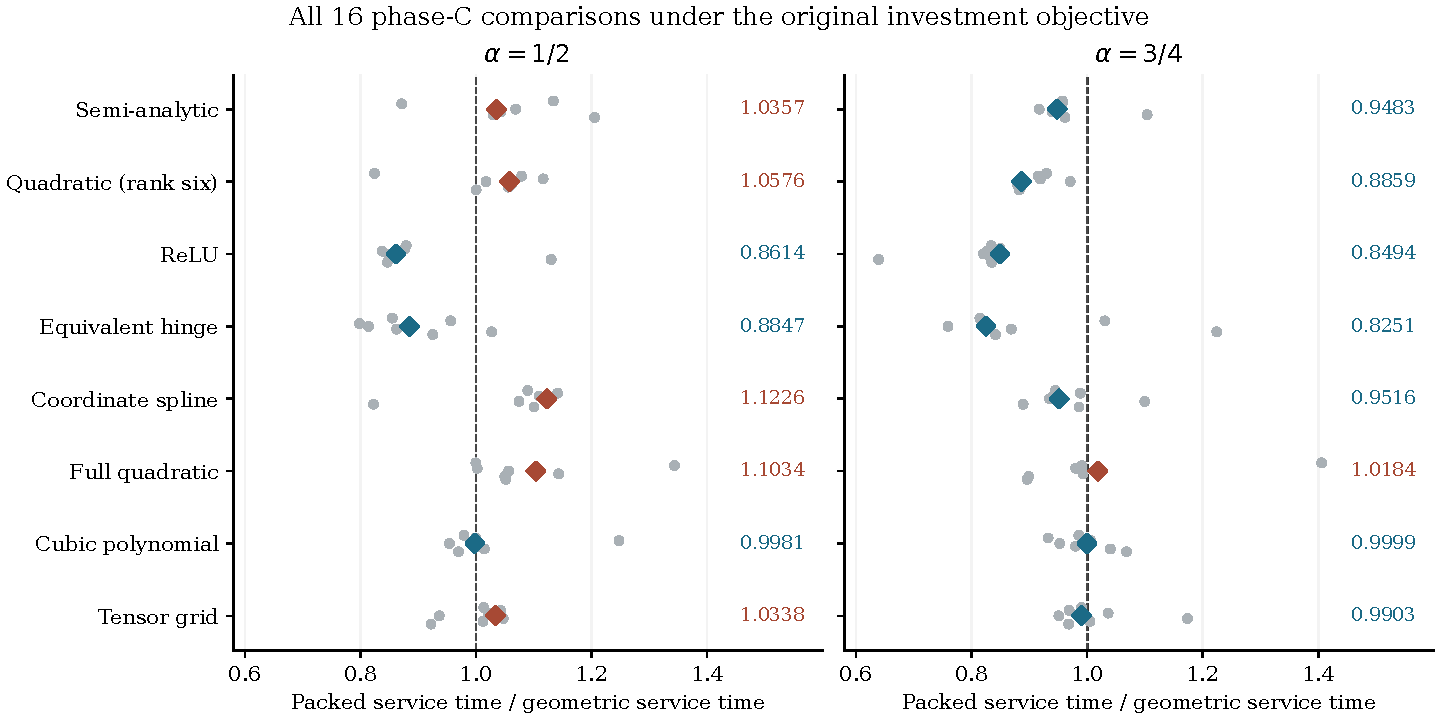
\includegraphics[width=\linewidth]{figures119/phase_c_all_clocks119.pdf}
\caption{All contemporaneous phase-C packed/geometric service comparisons.
Diamonds show the ratio of the two seven-process median times; grey points
show every paired process ratio. Values below one favor packing. These are
32-decision service clocks with actual loading and broader process costs
reported separately, not confidence intervals.}\label{fig:clocks119c}
\end{figure}

All 13,824 primary and 21,504 timing decisions completed.  The native
exact record audit passes 1,325,935 checks over 55,043 attempted
certificates; a separate read-only report verifies all 768 raw hashes
and 384,551 further exact/identity conditions.  An additional 21,974
read-only checks reconstruct the same original point coordinates for
the budgeted and fused services from their exact state, action, cut and
resolution records.  All 5,888 paired decisions use identical paid
preliminary information and qualification exits.  F uses 27 packed
compiler calls for the primary catalogue and 182 across the seven timing
processes, containing respectively 24,193 and 35,504 midpoint/endpoint
payloads.  The separate two-point defect calculation remains charged.
The 30-value general and 16-value boundary preliminary caps are attained
and respected.  Complete original risk-point queries remain 154,217,
exactly the budgeted service's count.

Table~\ref{tab:timing119c} reports the full contemporaneous comparison.
F is faster than B in all 16 median-clock cells, including 11 with all
seven paired clocks lower.  It is faster than C in all 16 medians, than
T in 14, and than G in ten.  The remaining six losses against G are
retained.  At $\alpha=1/2$, the ReLU ratio F/G is $0.8614$, with six
paired wins; at $3/4$ it is $0.8494$, with seven.  Conventional hinges
benefit similarly.  Quadratic at $1/2$ instead has ratio $1.0576$,
while quadratic at $3/4$ has ratio $0.8859$ and seven paired wins.
The degree-three polynomial ratios $0.9981$ and $0.9999$ illustrate
why a median win alone is weak evidence of a substantial advantage.
All ranges and every clock remain reported; no timing confidence
interval or architecture-independent speed guarantee is inferred.

Across all primary cells, F costs $6.5522$ seconds, compared with
$6.7726$ for G and $6.8250$ for B.  It is faster than G in 11 of 16
complete 144-state service cells and slower in five.  These totals
describe the entire predeclared tournament.  They do not construct a
new service by selecting the fastest implementation state by state.
The result identifies a practical part of the information-to-work
connection: the proved small payload budget becomes more competitive
when its many individual arrays are evaluated together.  Packing,
scattering, outward zero terms, attempted certificates and all fallback
work remain inside the measured boundary.

All fifteen within-arm service contrasts still have exactly the same
complete original policy at each of 2,304 state--risk--arm combinations.
Their original economic contrast is exactly zero.  Repacking changes
some outward endpoints---600 primary and 2,030 timing rows differ from
B---without changing their qualification exits or policies.  Original
regret and action-distance bounds retain their previous interpretation,
and no exact rational fallback is needed.  The 1,464 primary repairs
are the same 244 distinct proposals repaired under six services.

Representation-specific adoption remains unsupported.  Charging fresh
standalone acquisition and actual loading, quadratic with G costs
$0.1485$ seconds for the full $\alpha=1/2$ catalogue, versus $0.3407$
for ReLU with F.  At $3/4$, quadratic with F costs $0.1417$, versus
$0.3131$ for ReLU with F.  Quadratic also has the strictly lower
catalogue-mean original economic cost at both risks.  The ReLU--hinge
identity holds in all 96 paired files and 4,416 paired decisions,
including attempted certificates.  The conditional adoption inequality
in Section~\ref{sec:study119} therefore continues to require the full
resource and economic comparison, not an architecture label.  Phase C
adds a shared original-decision computational improvement while
preserving the negative A/B implementation findings, R97's adverse
acquisition result, and the still-open action-aligned learning and
larger-application obligations.

\subsection{Independent value enclosures for every recorded original policy}
\label{sec:study119d}
The 1,024-bin reference uses a separate whole-support risk partition with the
shared verified terminal compiler. To check original policy values through a
separate implementation, validation D was frozen at \texttt{cafd38ae}
after all A--C outcomes were known. It fixes 64 whole-support cells and up to 32
rational terminal bisections on every one of the 983 realized state/action/risk
keys represented by C's 13,824 primary decisions. The exact binary state and
action identities are retained. This is validation of the known catalogue.

The standard-library implementation reconstructs the original nonlinear
economic primitives, the terminal shock polynomial and its continuous AVaR
integral, and a feasible strong-convexity bracket for $V_1^*$. Conditional
Jensen bounds for $(V_1^*\circ F-\eta)_+$ and the repeated-endpoint secant
mixture give independent whole-support bounds for the original $Q$.
Proposition~\ref{prop:independentvalidation119} in the supplement proves these bounds.
Adding the unchanged $\beta 2^{-20}$ future-controller allowance once gives
the complete-policy $J$ enclosure. The production compiler is not imported.
This does not directly evaluate the deployed floating terminal controller or
independently determine the global date-zero regret optimum.

All 983 keys and 126,807 exact terminal contexts completed, with
652,774 recorded checks and no failed key.
The independent intervals overlap all 13,824 corresponding service intervals
and all 983 shared-compiler reference intervals. Overlap establishes
compatibility; it does not certify each fine reference endpoint merely from
intersection. All exact traces, checks and containment directions are retained.

\begin{table}[t]\centering\small
\caption{Independent Fraction original-policy mean-cost enclosures on the fixed catalogue.}\label{tab:independent119d}
\begin{tabular}{llrr}\hline
$\alpha$ & Representation & Lower mean cost & Upper mean cost \\ \hline
$1/2$ & Semi-analytic & 0.611452244 & 0.611454152 \\
$1/2$ & Quadratic (rank six) & 0.611604999 & 0.611606910 \\
$1/2$ & ReLU & 0.611623342 & 0.611625227 \\
$1/2$ & Equivalent hinge & 0.611623342 & 0.611625227 \\
$1/2$ & Coordinate spline & 0.611715940 & 0.611717849 \\
$1/2$ & Full quadratic & 0.611604999 & 0.611606910 \\
$1/2$ & Cubic polynomial & 0.611667314 & 0.611669224 \\
$1/2$ & Tensor grid & 0.611462422 & 0.611464314 \\
$3/4$ & Semi-analytic & 0.621104706 & 0.621106644 \\
$3/4$ & Quadratic (rank six) & 0.621266923 & 0.621268911 \\
$3/4$ & ReLU & 0.621285373 & 0.621287354 \\
$3/4$ & Equivalent hinge & 0.621285373 & 0.621287354 \\
$3/4$ & Coordinate spline & 0.621393664 & 0.621395613 \\
$3/4$ & Full quadratic & 0.621266925 & 0.621268914 \\
$3/4$ & Cubic polynomial & 0.621313002 & 0.621315001 \\
$3/4$ & Tensor grid & 0.621139623 & 0.621141543 \\
\hline\end{tabular}
\\[4pt]\parbox{.96\linewidth}{\footnotesize Each endpoint is an outward decimal display of an exact rational bound. Every mean weights the same 144 realized original states equally. All six services return exactly the same complete policy within an arm; all 96 arm/service/risk means are retained in the development companion. The future-controller allowance is $\beta 2^{-20}$. These intervals are numerical enclosures, not sampling confidence intervals.}
\end{table}


All 96 arm/service/risk means and all 56 arm contrasts are independently
reaggregated. There are 32 strictly negative, 20
strictly positive, 2 exact-zero and 2
unresolved contrast intervals in the fixed left-minus-right orientation.
The ReLU-minus-quadratic original mean-cost intervals are
$[17.4360, 19.2238]\times10^{-6}$
at $\alpha=1/2$ and
$[17.5331, 19.3595]\times10^{-6}$
at $\alpha=3/4$. The full contrast table retains every sign and exact tie.
These independent intervals confirm the rank-six quadratic arm has strictly lower mean original policy cost than ReLU at both risk levels. ReLU and its exactly equivalent conventional hinge representation retain identical realized policies and exact-zero mean cost contrasts.
All 240 arm/risk/service-pair cells have identical complete policies, preserving
the exact zero economic effect of changing only the certification service.
No favorable economic sign was a validation pass condition.

D requires 1697.332 seconds of additional actual
author-side validation time (1693.604 CPU seconds),
including its separately recorded binding, rational solves, primitive traces
and aggregation. This cost is reported separately from the unchanged A--C
acquisition and service clocks. D strengthens independent original-model value
evidence; it creates neither an unseen population result nor a neural-specific
adoption claim.

\section{Conclusion}\label{sec:conclusion119}
Neural Bellman Operators link recursively acquired continuations to feasible
original-objective decisions. The complete account includes the actor's own
future policy, action-dependent continuation error, original-law numerical
witnesses and the cost of obtaining them. The original construction and the
completed-policy safeguards establish precise decision guarantees without
assuming that an optimizer successfully trains an arbitrary network.

The present revision identifies the adverse innovation region as a paid
information decision. For scalar uniform risk and convex Lipschitz
continuations, locating that region before integration yields matching
deterministic bounds with linear tail-length dependence. The original
investment primitives turn an approximate location into an outward
all-action certificate, and a finite preliminary budget limits work spent
before the complete original solver is invoked. These contributions concern
the information and certification components of NBOs and are available to
all same-information representations.

The experiments distinguish information savings, service time and economic
loss. They retain every fixed-catalogue decision, every timing repetition,
all rejected certificates, independently paid references and the strong
conventional frontier. Equivalent ReLU and hinge actors receive equal
information and full acquisition charges. An unchanged complete policy has
unchanged original economic value. Computational adoption therefore requires
both a competitive complete service and a justified economic workload; a
smaller fitting residual or a smaller query count alone does not establish it.

The research program continues toward prospective action-aware acquisition,
neural-specific benefits under matched resources, larger dynamic economic
problems and calibrated use. The new proofs and executed algorithms make
those questions more sharply testable. The complete supplement states the
mathematical assumptions and proofs, while the development companion retains
the earlier applications, policy improvements, negative experiments, unresolved
claims and independent source identities needed to continue that program.

\bibliographystyle{ecta-fullname}
\bibliography{references99,references110-additions}
\end{document}
